\variant
\\
\begin{minipage}[t]{3.25in}
An I-beam is going to carry vertical load in a building, and mounted to fix both the top and bottom of the beam against rotation (left configuration). However, the load on beam was found to be very close to the critical load for buckling. To improve safety, additional horizontal I-beams were added to act as pin-supports to the middle of the beam (right configuration), for both in the page and out of the page directions. What is the  critical load of the right configuration compared with the critical load of the left configuration?
\end{minipage}
\quad
\begin{minipage}[t]{2.75in}
\vspace{-12pt}
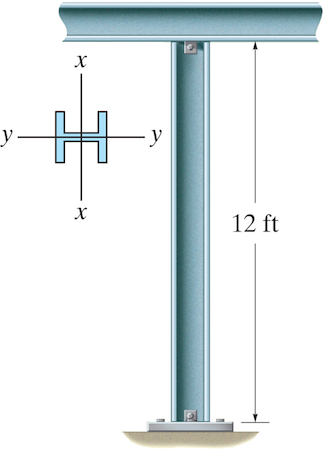
\includegraphics[height=2in]{ch17-ibeam-vert}
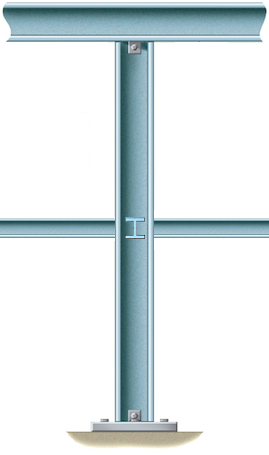
\includegraphics[height=2in]{ch17-ibeam-vert-support}
\end{minipage}
%\vspace{-48pt}
\begin{answers}
\answer $P_\text{cr}(\text{right}) = 4 P_\text{cr}(\text{left})$
\answer $P_\text{cr}(\text{right}) = (4\times 0.7^2) P_\text{cr}(\text{left})$
\answer $P_\text{cr}(\text{right}) = (0.7^2) P_\text{cr}(\text{left})$
\correctanswer $P_\text{cr}(\text{right}) = (1/0.7^2) P_\text{cr}(\text{left})$
\answer $P_\text{cr}(\text{right}) = (4/0.7^2) P_\text{cr}(\text{left})$
\end{answers}
\begin{solution}
The left configuration has an effective length of $L/2$ ($L = 12\text{ ft}$) as it is fixed at both ends. The right configuration has an effective length of $0.7 L/2$, as it is fixed at the bottom and pin-connected at half the height. Then, the critical loads are
\[
P_\text{cr}(\text{left}) = \frac{\pi^2 EI}{(L/2)^2} = 4\frac{\pi^2 EI}{L^2}
\]
and
\[
P_\text{cr}(\text{right}) = \frac{\pi^2 EI}{(0.7 L/2)^2} = \frac{4}{0.7^2} \frac{\pi^2 EI}{L^2}
\]
So, the right configuration has a critical load that is $(1/0.7)^2 \approx 2$ times larger than the left configuration.
\end{solution}

